\documentclass[italian,10pt,a4paper]{report}
\usepackage[utf8]{inputenc}
\usepackage[T1]{fontenc}
\usepackage{babel}
\usepackage[hidelinks]{hyperref}
\usepackage{graphicx}
\usepackage{amsmath}
\usepackage{multicol}
\usepackage{listings}
\usepackage{color}

\definecolor{dkgreen}{rgb}{0,0.6,0}
\definecolor{gray}{rgb}{0.5,0.5,0.5}
\definecolor{mauve}{rgb}{0.58,0,0.82}

\lstset{frame=tb,
	language=Java,
	aboveskip=3mm,
	belowskip=3mm,
	showstringspaces=false,
	columns=flexible,
	basicstyle={\small\ttfamily},
	numbers=left,
	numberstyle=\tiny\color{gray},
	keywordstyle=\color{blue},
	commentstyle=\color{dkgreen},
	stringstyle=\color{mauve},
	breaklines=true,
	breakatwhitespace=true,
	tabsize=4
}

\graphicspath{img}
\title{Appunti di Big Data}
\author{Riccardo Torre}
\begin{document}
	\maketitle
	\tableofcontents
	\chapter{Introduzione}
	Attenzione. Questi appunti non sono un sostituto delle lezioni. Il programma del corso potrebbe variare, attenersi alle disposizioni del docente.
	\section{Big Data: cos'è?} Il termine Big Data nasce con l'Internet 2.0 e può essere definito in modi diversi. Lo si può definire come "un grande insieme di dati eterogeneo la cui dimensione, diversità e varietà deve essere gestita in maniera tale da estrarne valori/significati". I Big Data hanno le seguenti caratteristiche:
	\begin{itemize}
		\item Volume, ovvero la quantità dei dati;
		\item Varietà, ovvero il tipo di dato;
		\item Velocità, ovvero la velocità con cui vengono generati i dati.
	\end{itemize}
	A queste se ne sono aggiunte nel tempo altre due:
	\begin{itemize}
		\item Valore, ovvero che i dati contengano info che mi interessa estrarre;
		\item Veridicità, ovvero che la fonte dei dati sia verificabile.
	\end{itemize}
	%-----------------------
	I dati vengono prodotti dall'attività degli utenti su Internet (social media, piattaforme per la condivisione di video, piattaforme streaming, musica, giochi, ecc\dots). 
	Gli approcci alla programmazione su singola macchina e alla programmazione parallela non sono adatti (poca scalabilità).
	
	Questo corso presenta i modelli di programmazione che supportano il calcolo distribuito.
	\begin{itemize}
		\item Non mi interesa scalare verticalmente (incrementare la potenza di una macchina) bensì vado ad affiancare macchine con le stesse caratteristiche (scalabilità orizzontale;
		\item i guasti sono la norma; almeno un guasto al giorno in un \textit{cluster};
		\item lo storage è distribuito; il processing è distribuito, tiene conto della località del dato (questo per risparmiare banda);
		\item il processing viene fatto tutto insieme; l'analisi parallela deve essere il più trasparente possibile all'utente: cioè l'utente non deve accorgersi che dietro c'è parallelismo. Il modo di programmare cambia, ma non deve essere l'utente a gestire i guasti (è il sistema che deve gestire lo scheduling del processing per fare fronte ai guasti).
	\end{itemize}
	\section{Panoramica sull'architettura - lab}
	Su una singola macchina sono presenti:
	\begin{itemize}
		\item cpu
		\item memoria
		\item disco
	\end{itemize}
	Quando si ha a che fare con una grande quantità di dati si utilizza un insieme di server raggruppati in "armadi" (in inglese \textit{rack}).
	
	\begin{figure}
		\centering
		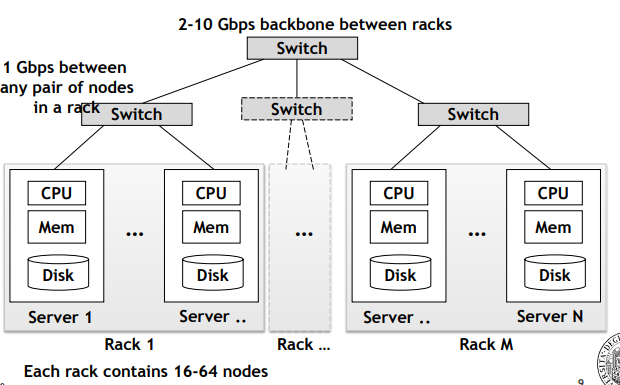
\includegraphics[width=0.7\linewidth]{img/racks}
		\caption{architettura di riferimento}
		\label{fig:racks}
	\end{figure}

	I server tra armadi diversi comunicano tramite gli switch (guardare figura \ref{fig:racks}). Gli switch sono il collo di bottiglia perché il numero di porte è limitato. Lo strumento principale per gestire il calcolo distribuito è \textbf{Hadoop}: può essere visto come un sistema operativo (perché gestisce le risorse di memorizzazione, di calcolo) che offre all'utente un'interfaccia per gestire le operazioni (del calcolo distribuito). Permette di gestire le CPU e le risorse di memorizzazione su disco.
	Il file system è distribuito e si chiama HDFS (\textit{Hadoop Distributed File System}). Il file viene distribuito in blocchetti come in figura \ref{fig:hdfs}
	\begin{figure}
		\centering
		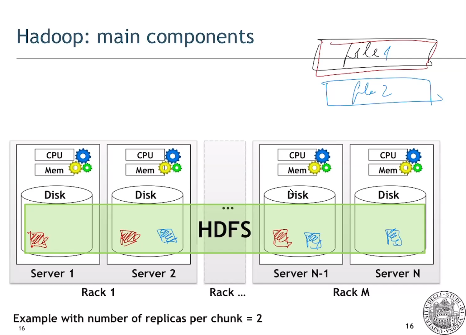
\includegraphics[width=0.7\linewidth]{img/hdfs}
		\caption{hdfs come file system distribuito}
		\label{fig:hdfs}
	\end{figure}
	Prima di mandare in produzione sul cluster\footnote{il cluster è un insieme di computer connessi tra loro tramite una rete telematica} si effettuano dei test in locale lanciando il sistema su una singola macchina.
	
	\section{Word count}
	N.B: questa è una versione semplificata dell'algoritmo word count.
	Abbiamo una collezione ampia di testi da analizzare all'interno di una directory di Hadoop. Vorremmo contare il numero di occorrenze delle parole (dizionario chiave valore). 
	\begin{figure}
		\centering
		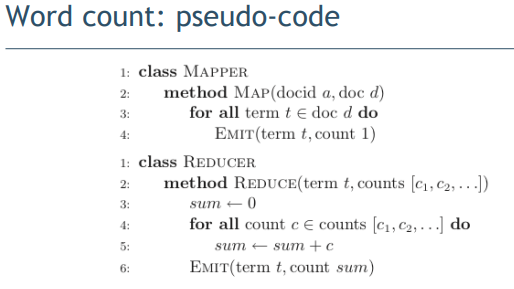
\includegraphics[width=0.7\linewidth]{img/pseudocodice-word-count}
		\caption{presudocodice del word count}
		\label{fig:pseudocodice-word-count}
	\end{figure}
	\begin{figure}
		\centering
		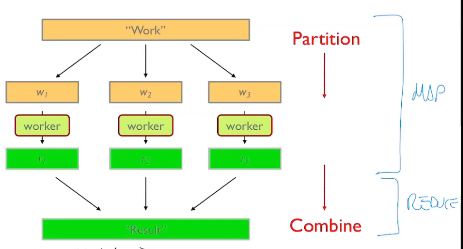
\includegraphics[width=0.7\linewidth]{img/divide-and-conquer}
		\caption{fase map (sopra) e fase reduce (sotto)}
		\label{fig:divide-and-conquer}
	\end{figure}
	
	Ci sono due fasi (guardare figura \ref{fig:pseudocodice-word-count} e figura \ref{fig:divide-and-conquer}): 
	\begin{itemize}
		\item fase \textbf{map}: calcolo distribuito, gestito dalla classe \textit{mapper}. Il metodo prende in input un \textit{id} del documento da analizzare e il \textit{percorso} relativo al documento (riga 1). Il ciclo for alla riga 3 e 4  aggiunge una copia chiave-valore, dove la chiave è una parola (term) presente nel documento e il valore è il conteggio delle occorrenze della chiave (term).
		\item fase \textbf{reduce}: aggregazione dei risultati parziali in un unico risultato, gestito dalla classe \textit{reducer}. Il metodo reduce prende in input un termine (o parola) e i conteggi di tutte le occorrenze di quel termine (provenienti dai vari workers che hanno letto ciascuno un sottoinsieme dell'insieme di file passato all'inizio dell'elaborazione), inizializza una variabile locale sum a zero (linea 3) e per ogni conteggio nella lista dei conteggi, aggiorna la somma per quel termine e al termine del ciclo inserisci nella mappa risultante, il conteggio trovato (conteggio finale).
	\end{itemize}
	Il processo descritto nella figura \ref{fig:divide-and-conquer} è trasparente al programmatore, nel senso che viene gestito in maniera autonoma dal framework. In altre parole il programmatore non si deve occupare di gestire la suddivisione del work e l'aggregazione del risultato.
	\begin{figure}
		\centering
		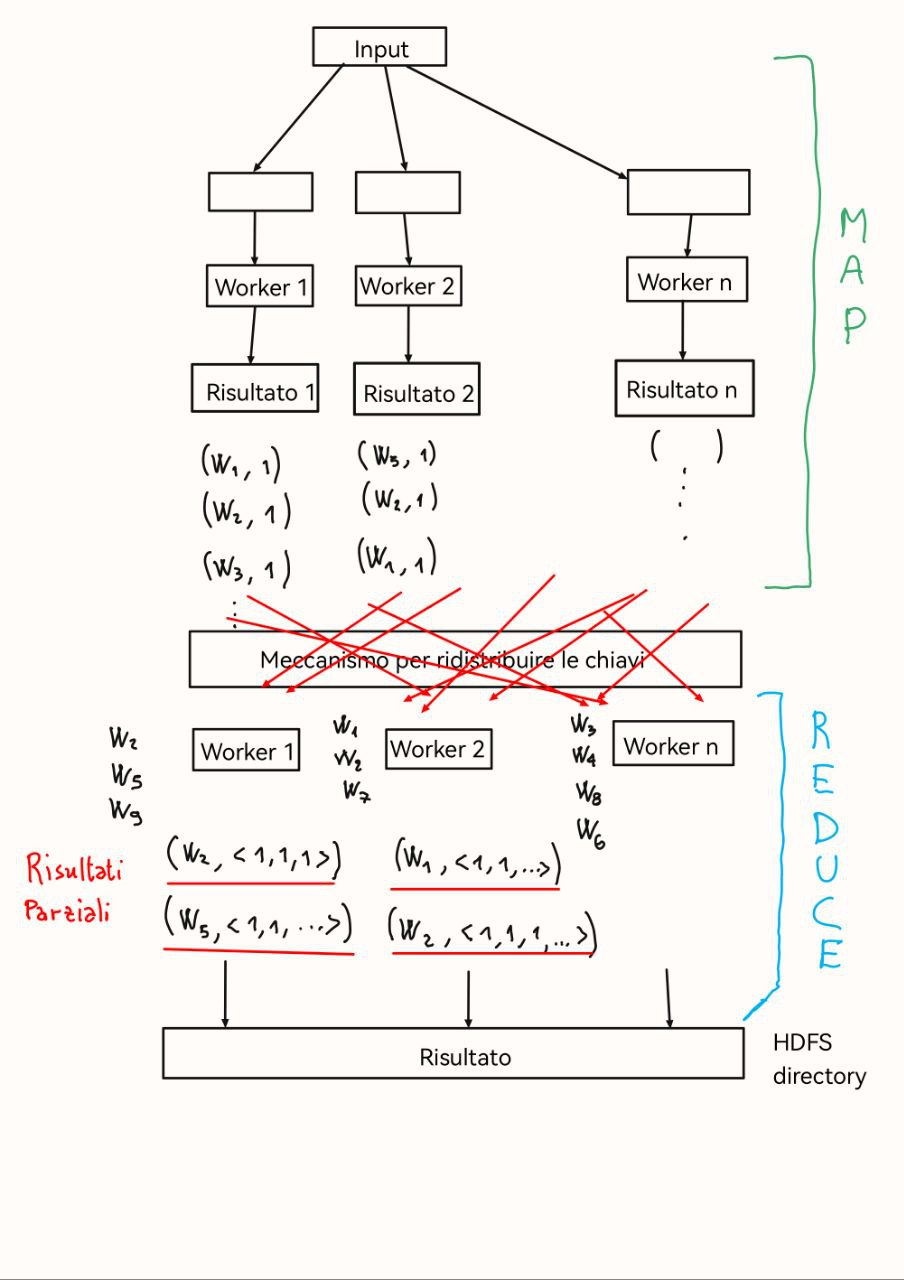
\includegraphics[width=\linewidth]{img/map-reduce-tablet}
		\caption{processo map reduce}
		\label{fig:map-reduce-tablet}
	\end{figure}
	La programmazione funzionale viene utilizzata nel modello map reduce. Facendo riferimento alla figura \ref{fig:pseudocodice-word-count} nel codice del mapper, alla riga 4 viene fatto un emit, che consiste nell'azione di scaricare il worker i-esimo (figura \ref{fig:map-reduce-tablet}) e costruire il risultato. Ad esempio il worker 1 produce il risultato 1 che è composto dal conteggio ($w_1$,1), ($w_2$,1), \dots e questo conteggio, scarica il worker 1 ma carica la memoria (ma questo mi permette comunque di risparmiare rete). In MapReduce viene utilizzato molto la struttura dati mappa. 
	
	Il programmatore definisce un mapper e un reducer come segue:
	\begin{align*}
		&map \colon (k_1,v_1)\xrightarrow{}\left[(k_2,v_2)\right]\\
		&reduce \colon (k_2,\left[v_2\right]) \colon \left[(k_3,v_3)\right]
	\end{align*}
	map prende in ingresso una coppia chiave-valore e restituisce una struttura dati mappa che contiene le coppie chiave-valore. Reduce invece prende una chiave e una struttura dati contenente i relativi valori e restituisce la coppia chiave-valore relativa all'operazione effettuata sui dati aggregati.
	Per distribuire le chiavi tra i vari worker (nel livello reduce nella figura \ref{fig:map-reduce-tablet}) l'opzione di default è una distribuzione casuale basata su hash che può essere ottenuta facendo un hash sulla chiave e applicando al risultato il modulo del numero di lavoratori. Quindi una chiave $i$ verrà sempre applicata allo stesso lavoratore. L'ordine è legato al tipo di dato (metodo compare di Java che varia da tipo a tipo, ad esempio String, Integer, \dots). In alcuni casi, risulta necessario applicare l'operazione map reduce più di una volta. I risultati intermedi della fase di map, non vengono eliminati fino a quando non viene completata anche la fase di reduce (dunque se si interrompe il processo, si può riprendere ad eleborare a partire dai risultati intermedi).
	\newpage
	\section{Il framework Hadoop}	
	Il linguaggio in cui è stato scritto il framework è Java. Le classi principali di Hadoop sono le seguenti.
	\begin{itemize}
		\item Writable: definisce una serializzazione/deserializzazione del protocollo. Ogni tipo in Hadoop è della classe Writable
		\item WritableComparable: classe che estende Writable e che implementa il metodo compareTo di Java. Si può quindi definire un ordine sugli oggetti di questa classe.
		\item classi che estendono WritableComparable e che sono da utilizzare al posto dei tipi non primitivi di Java (ad esempio: Integer, String, Boolean, ecc\dots); per esempio IntWritable, LongWritable, Text, e così via\dots
	\end{itemize}
	L'utente vede solo gli oggetti specifici di Hadoop (mentre durante l'elaborazione, il framework può utilizzare i tipi di Java). \textbf{Nota:} non esiste un corrispettivo tipo del framework per ogni tipo Java. È il programmatore che deve costruire tipi più complessi (quando il framework non può offrire tipi).
	Un Mapper viene costruito come segue:
	\begin{verbatim}
		void map(k1 key, v1 value, Context context)
	\end{verbatim}
	dove context è il contesto in cui viene creata la mappa. Il framework prende il file di input e lo suddivide in record da dare a ciascun mapper. Se dobbiamo lavorare con i dati in ingresso si utilizzano classi basate su InputFormat. Ad esempio TextInputFormat prende un file, lo suddivide tra diverse macchine. Ciascuna macchina restituisce una coppia chiave-valore, dove la chiave è l'offset a cui si trova quella riga specifica e il valore è la riga stessa. Ad esempio preso il testo 
	\begin{multicols}{2}

			\begin{verbatim}
				1: On top of the Crumpetty Tree
				2: The Quangle Wangle sat,
				3: But his face could not see,
				4: On account of his Beaver Hat
			\end{verbatim}
			\columnbreak
			\begin{verbatim}
				(0,On top of the Crumpetty Tree)
				(33, The Quangle Wangle sat,)
				(57, But his face could not see,)
				(39, On account of his Beaver Hat)
			\end{verbatim}			
	\end{multicols}
	Nella colonna di destra le tuple contengono la chiave che è un valore di tipo IntWritable e un valore di tipo Text.
	
	\chapter{Progettazione di algoritmi e strutture dati}
	\chapter{Laboratorio con Hadoop}
	\section{Lab 1}
	\lstinputlisting[label=code:wordcount, caption={classe WordCounter}]{WordCount.java}
	Le classi che sono d'interesse maggiore:
	\begin{itemize}
		\item La classe \textbf{Map} (linee 44-55) estende Mapper;
		\item La classe \textbf{Reduce} (linee 57-70) estende Reducer.
	\end{itemize}
	\newpage
	
		\subsection{Analisi di Map}
		Fare riferimento al codice \ref{code:wordcounter-map}.
		\lstinputlisting[firstline=39,lastline=55,label=code:wordcounter-map,caption=classe Map di WordCount]{WordCount.java}
		\begin{itemize}
			\item (LongWritable, Text): è la coppia chiave-valore in input al Mapper (che è il file di testo da analizzare). Il file viene suddiviso in righe dal FileInputReader e invia ciascuna riga al Mapper. LongWritable (chiave) è l'offset della riga rispetto all'inizio del file e Text (valore) è la riga da analizzare che viene passata al Mapper.
			\item (Text, IntWritable): è la coppia chiave-valore in output dal Mapper. Text corrisponde ad una parola della riga da conteggiare e che è stata precedentemente passata in input. Il valore è il conteggio della parola (restituisce 1 nel caso che andiamo a considerare perché non è nel nostro interesse salvare risorse).
		\end{itemize}
		
		Il metodo map (linea 1) ha una firma formata da:
		\begin{itemize}
			\item LongWritable offset: corrisponde all'offset a cui si trova la linea da analizzare rispetto l'inizio del file;
			\item Text lineText: la linea passata al mapper e da analizzare, e appartenente all'insieme delle linee che compongono il file di testo originale;
			\item Context context: permette di comunicare correttamente con il framework.
		\end{itemize}
		Nella linea 2 viene dichiarata una costante istanziata a tempo di compilazione che contiene il valore 1 ed è del tipo IntWritable.
		Nella linea 3 viene creata una variabile di tipo Text che conterrà il valore della parola estratta dalla linea corrente. Nella linea 4, viene utilizzato un oggetto di tipo Pattern, il cui scopo è di catturare le stringhe che rispettano l'espressione regolare specificata nella chiamata di metodo compile. Vengono specificati due backslash seguito da una lettera, ciascuna con un proprio significato. La lettera \textit{s} indica uno spazio, la lettera \textit{b} indica un "word bound" che corrisponde alla posizione di inizio o di fine di una parola. L'asterisco significa zero o più caratteri.
		
		Alla linea 7 viene salvato il valore di lineText (di tipo Text) in un tipo String. È importante ricordare che non possono essere utilizzati i tipi del framework nell'implementazione dell'algoritmo. Questo segue l'idea di lasciare al programmatore il compito di implementare solamente nel linguaggio familiare di Java (e non quello del framework) le funzionalità delle classi Map e Reduce.
		
		Nelle linee successive (6-14) viene utilizzato l'oggetto Pattern WORD BOUNDARY per estrapolare dalla linea corrente (line) le parole che la compongono, facendo attenzione a controllare che siano diverse dalla stringa vuota. Notare che 
		\begin{lstlisting}
			WORD_BOUNDARY.split(line)
		\end{lstlisting}
		dentro al foreach restituisce un iteratore sulla lista di parole che compongono la linea corrente.
		La parola corrente viene dunque salvata dentro currentWord (linea 12) e viene fatto "l'emit" della stessa con il valore del conteggio ad uno (linea 13).
		Fare l'emit significa restituire chiamare il metodo write sull'oggetto context (corrisponde a restituire il risultato dell'oggetto Map al framework).
		
		\subsection{Analisi di Reduce}
		\lstinputlisting[label=wordcounter-reduce, caption=classe Reduce di WordCount, firstline=56,lastline=69]{WordCount.java}
		Fare riferimento al codice \ref{wordcounter-reduce}
\end{document}	